\chapter{Desarrollo de software}\label{S:tema_4}
Para el desarrollo de software de una manera adecuada, profesional e interdisciplinar (independiente de lenguaje, framework o grupo de trabajo) es necesario no solo unas herramientas en común, sino unas dinámicas de trabajo en equipo y especialmente una metodología de trabajo técnica, profesionalizada.

Usualmente se entiende que aunque un autónomo o freelance desarrollan un trabajo adecuado, en software el review o validación por terceros es un elemento crítico en la filosofía de verificación mejora y calidad del producto por ello asumimos que el entorno de trabajo cuenta siempre con un mínimo de 3-4 personas que forma un equipo técnico.

Por otra parte el equipo asume que tanto las tareas a realizar como la responsabilidad de las mismas no es personal sino grupal, por lo que todo el equipo debe ser involucrado en las tareas de gestión, desarrollo, testeo, documentación y puesta en marcha de la aplicación.

\section{Dinámica de trabajo (equipo)}
Actualmente por contexto laboral, las filosofía de trabajo AGILE\cite{c_agile}, y en concreto SCRUM\cite{c_scrum} son de amplia aceptación y exitosas. Por ello son las seleccionadas por este documento.

\subsection{Agile}
Agile es una metodología de trabajo cuya principal enfoque reside en la gestión de equipos y proyectos; define la manera de interaccionar personas, herramientas y procesos favoreciendo la colaboración con el cliente por encima de la negociación contractual. Su principal objetivo es el desarrollo de software funcional y la flexibilidad o respuesta al cambio a la hora de seguir una planificación.

\begin{figure}[!htb]
\begin{center}
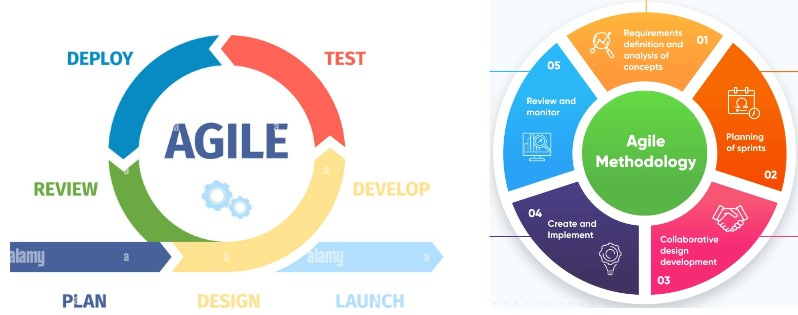
\includegraphics[width=1\textwidth]{./figuras/agile}
\caption{Diagrama metodología AGILE.}
\label{F:agile}
\end{center}
\end{figure}

\subsection{Scrum}
Scrum es la implementación de una filosofía agile, destaca por su aproximación en fases y división del tiempo de trabajo en sprints (2-3 semanas de trabajo). El objetivo de scrum es la mejora continua, facilitando el valor añadido en un calendario de entregas, para ello define unas fases de planificación, evaluaciones diarias, re-definición, review y retrospectiva. Existen roles como el product owner que interacciona con los clientes para garantizar que se entienden los requisitos y se alcanzan los objetivos marcados para cada sprint. El equipo utiliza las “historias” del cliente-product owner, para definir tareas funcionales, estas deben ser especificadas y estimada por el equipo dentro de un backlog.

\begin{figure}[!htb]
\begin{center}
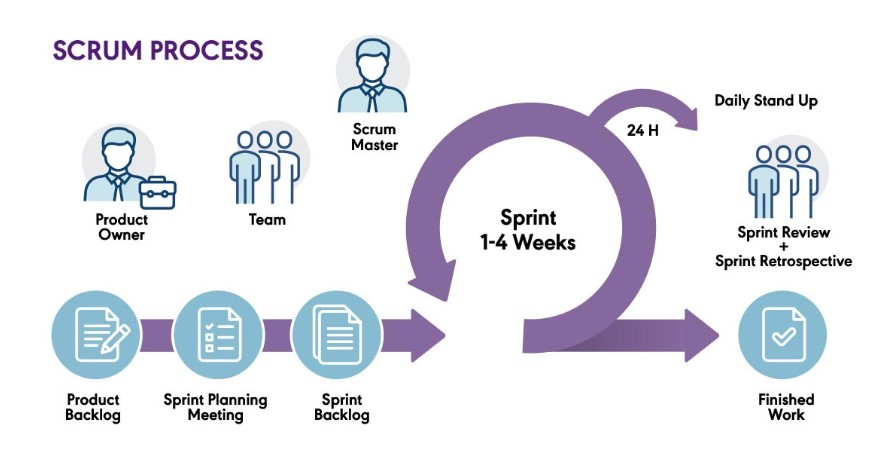
\includegraphics[width=1\textwidth]{./figuras/scrum}
\caption{Diagrama funcionamiento SCRUM-AGILE\cite{i_scrum}.}
\label{F:scrum}
\end{center}
\end{figure}
El scrum master es el encargado de facilitar y supervisar el funcionamiento del scrum, dirigiendo las reuniones. El y el equipo planifican los tickets a realizar en un sprint, entre los estimados del backlog. Diariamente se comenta brevemente el trabajo realizado, problemas abordados del día anterior y la previsión diaria.

En caso de cambios no planificados se re-priorizan los tickets y se redefine el sprint restante, con el fin de obtener siempre una mayor satisfacción en la entrega. Una vez acabado el sprint, se realiza un proceso de review con el cliente con feedback real y de calidad sobre el resultado obtenido así como una retrospectiva del equipo sobre que se hizo bien, mal, causas, mejoras a implementar especialmente desde el punto de vista de gestión e información dentro del equipo.

Desde el puntos de vista técnico, cada cambio no solo está traceado por un ticket del sprint, sino que debe incluir las siguiente apartados:
\begin{itemize}
    \item Documentación, descripción técnica de los cambios realizados por la tarea, que fundamenta la documentación general del software.
    \item Pull request, con el código de la tarea, auto-explicativo o apropiadamente documentado. Todo código debe respetar un código de buenas prácticas general o definido por el equipo. Test unitario o de integración que validan la funcionalidad añadida.
    \item Validación de un CI build con revisión aprobada, donde se compila ejecuta los test, se pasa validadores de calidad de código o vulnerabilidades como sonar\cite{c_sonar} o blackduck\cite{c_blackduck}. Review cualitativo de otros programadores y review en profundidad por aquellos que conocen la naturaleza del servicio o los cambios (approved).
\end{itemize}

\subsection{Generalización y profesionalidad}
La importancia tanto de la metodología de equipo, como las buenas prácticas y estructuras de trabajo no solo aporta robustez, calidad y estandarización al trabajo entregado, sino que permite optimizar al equipo como cadena de trabajo.

 Un caso destacado del trabajo estandarizado es la generalización de tareas, es decir, cualquier elemento del equipo puede asumir o traspasar tareas aunque no sean suyas, ya que el código debe ser fácilmente legible, testeado y documentado; fielmente protocolizado. Y este punto normalmente es inviable en equipos inferiores a 3-4 personas, donde no hay una dinámica de trabajo en equipo, sino división del trabajo y asignación de elementos.

Por ello la transferencia de tareas/código tienden a generar refactorizaciones o recreaciones de software ante la inviabilidad de mantenimiento o comprensión por ser un software no estandarizado o dicho de otra forma, creado por desarrolladores que no saben trabajar en equipo, o no profesionalizan su trabajo ya que no puede ser transferido.

\section{Git, CI/CD y contenedor}
Actualmente toda empresa de software debe de tener un control sobre los cambios del software y mecanismos automatizados para la evaluación del mismo. Pasar código por mail, usb o un almacenamiento en la nube no solo es un riesgo de seguridad sino que no es profesional y es el principio de un ciclo de malas praxis.

\subsection{Git y repositorios de código}
Git\cite{c_git} es un programa de control de versión, significa que define versiones de código, permite generar nuevas versiones cuando se le generan cambios al código. 

Permite calcular las diferencias entre versiones del código anterior y realizar “commits”, es decir, aglutinar un conjunto de cambios y almacenarlos como diferencias entre la versión anterior y nueva. Este commit, incluye un mensaje descriptivo de los cambios y en muchas ocasiones código o nombres del ticket asociado para trazabilizar el cambio.

El código se construye desde un commit inicial a la versión deseada, esta aplicación de las diferencias, permite la generación de “ramas” en base a aplicar unos cambios u otros. 

El concepto de rama permite establecer versiones en paralelo del mismo software, así mismo permite unir ramas (merge) o crear nuevas a partir de las anteriores.
\begin{figure}[!htb]
\begin{center}
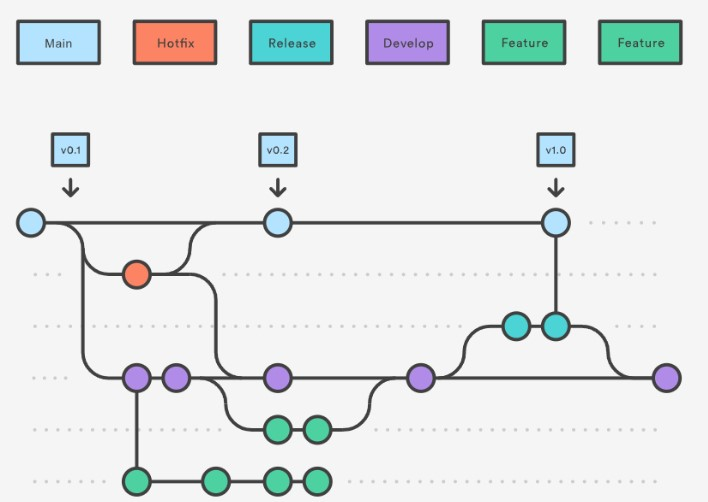
\includegraphics[width=1\textwidth]{./figuras/git_flow}
\caption{Diagrama flujo de trabajo en git\cite{i_git_flow}.}
\label{F:git_flow}
\end{center}
\end{figure}
 El verdadero potencial de este software es un repositorio o servidor git en línea, el concepto es sincronizar nuestro git local con repositorios en remoto que también sincronizan con otros desarrolladores de software. 
 
 Establecida una dinámica de trabajo (git flow figura \ref{F:git_flow}), permite trabajar de manera paralela a programadores sobre el mismo código sin “pisarse” y sobre todo, tracear y poder volver a versiones anteriores del código, sean nuestras o de otros desarrolladores.
 
\subsection{CI/CD}
CI/CD se refiere a las siglas de Integración Continua / Entrega Continua en inglés, es un concepto que se basa en el uso del repositorio de git y un código apropiadamente testeado.

Cuando se termina una tarea, el desarrollador realiza un PR (Pull Request) que inicia una petición de revisión de los commits añadidos para la funcionalidad, esta petición acciona un programa agente, que compila y ejecuta los test. Si es satisfactorio almacena la nueva versión del código compilado en un repositorio no de código sino de binarios/paquetes (según sea el lenguaje utilizado) y espera el 'ok' de otros programadores en el PR. Esta acción de construcción y testeo continuada de versiones del software o integración (CI), puede ser acompañada de script automatizados que despliegan (CD) directamente el software construido en una plataforma de trabajo, que puede ser desarrollo, test o directamente producción, es decir, continuamente se entregan versiones nuevas del software.

Como último eslabón, tenemos la 'contenerización' que en nuestro caso de uso es dockerizacion, es decir, generar un contenedor docker con los binarios generados por el CI y guardar la imagen en un repositorio de contenedores, para que el CD únicamente tenga que actualizar la imagen docker vieja por una versión más nueva en nuestro orquestador de despliegue.

\subsection{Opinión de un usuario con experiencia}
La combinación de un equipo agile con un entorno de git + CI/CD, más el uso de contenedores, permite el desarrollo en paralelo y revisión de tareas fácilmente, donde en cada cambio se valida el software y construye una nueva imagen, se despliega automáticamente sin riesgo humano. Todo ello con los beneficios intrínsecos mencionados que aporta docker a un software.

En mi opinión, este proceso completo únicamente se da en grandes empresas o startups tecnológicas con personal cualificado, pero en más del 50 \% de las pymes relacionadas con software o pequeños departamentos de software de grandes empresas, falla estrepitosamente, es decir, o no se aplica al completo o no se quieren aplicar tanto las metodologías de equipo o las automatizaciones y requisitos técnicos.

\section{CI basado en docker}
Históricamente se ha evolucionado desde un CI/CD de binarios, hacia un CI de binarios, que se construyen en un contenedor y el CD usa directamente el contenedor.

 El caso más utilizado jenkins\cite{c_jenkins}, es un agente multi-plugin que permite prácticamente la ejecución de cualquier lenguaje de programación, orquestador de dependencias y el uso  de terceras aplicaciones. El problema reside en que el agente debe tener acceso a máquinas con el compilador, máquina virtual o dependencias necesarias para la compilación y ejecución de los test. Al igual que un servidor linux, requiere de un mantenimiento y complejidad a la hora de gestionar adecuadamente las versiones y compiladores; especialmente cuando una empresa cuenta con múltiples equipos donde cada uno con un producto que puede tener requisitos diferentes.

 Una primera solución es el uso de docker como “aplicación”, es decir, utilizar los binarios de un container para ejecutar comandos específicos utilizando el directorio de trabajo como volumen. Así, una ejecución de maven/gcc/node/composer para generar los binarios/archivos necesarios y/o permite ejecutar los test. En dicho caso se reduce el mantenimiento, pero requiere de múltiples imágenes docker en el agente-ci.

En nuestro caso de interés, no disponemos de servidores-agentes sino que nuestra intención es que un container docker ejerza de agente-ci y por definición un container debe ser ligero. El punto novedoso, es el uso de container, con docker instalado, es decir, Docker in docker\cite{c_dind} y build ci\cite{c_ci_docker} en dockerfile con múltiples\cite{c_docker_multistage} etapas. Véase anexo \ref{S:docker_complex} docker desde dentro del propio contenedor. 

El segundo elemento es el uso de construcción de contenedores como build, es decir, compilar, ejecutar los test y construir la imagen en un único paso. Para ello se usa el concepto de múltiples etapas\cite{c_docker_multistage} que permite ejecutar pasos previos en imágenes base diferente que no son usadas para la imagen base final sino para la ejecución de comandos intermedios. 

Finalmente obtenemos que con solo docker instalado y la apropiada configuración, aquellos requisitos técnicos serán descargados como imágenes auxiliares usadas, y generan una imagen docker ligera únicamente con los ficheros necesario para la ejecución en producción.

\section{CI/CD dentro de nuestra nube}
Durante la realización de este documento se han realizado múltiples pruebas de concepto, entre ellas las prueba de un CI/CD basado en gitea\cite{c_gitea}-drone\cite{c_drone}. Al evaluar lo junto a servicios públicos externalizados como github\cite{c_github}, bitbucket\cite{c_bitbucket} o gitlab\cite{c_gitlab} entendemos que para un grupo reducido de desarrolladores es mas práctico y evita tareas de mantenimiento y segurización el uso de herramientas gratuitas externas. Sin embargo en aquellos casos donde el grupo de trabajo sea mas extenso o la naturaleza del código a generar tenga un carácter confidencial, se puede utilizar las pruebas conceptuales (véase anexo \ref{S:ci_ejemplo}) como parte de nuestra nube privada.

\section{Setup Software Local}
En los entornos locales puede haber una mayor diversidad de SO, ya que no es un elemento crítico para el desarrollo. Sin embargo debe existir una automatización y especialmente una estandarización con el objetivo de minimizar problemas o la no reproducción de circunstancias a la hora de depurar o corregir un error detectado en producción, por lo tanto es de especial interés que las versiones y software esté alineado no solo en producción sino entre los propios programadores (herramientas auxiliares). En los siguientes apartados se detallan las estrategias principales utilizadas como software-local para cliente de nuestra nube o herramientas y configuraciones de desarrollo.

\subsection{Automatización Local}
Podemos usar Scripting, principalmente bash o batch, aunque se recomienda el uso de ansible apuntado a localhost. Podemos distinguir varias tareas:
\begin{itemize}
    \item Instalación y configuraciones de elementos críticos de la compañía tales como cliente vpn, software de comunicaciones, correo o agentes de IT.
    \item Instalación de software necesario. Git, un gestor de repositorios git visual, compiladores, máquinas virtuales, IDE (Entornos de desarrollo), docker.
    \item Configuración de herramientas, gitignore, estandarización de IDE, puede ser definidas por la compañía, el grupo de trabajo o simplemente personalización individuales como los alias, guardadas en un repositorio de dot files.
\end{itemize}

\subsection{Herramientas de desarrollo basadas en docker}
Docker como compañía y empresa esta potenciando últimamente el segmento 'escritorio', especialmente en windows. Aunque docker CE (community edition) es open source, existe una versión privada con tools, interfaz gráfica y extras, dicha versión tiene engine para servidores y engine utilizada habitualmente en escritorio windows.

De una manera muy similar a la "dockerización de servicios", su intención es la dockerización de todo tipo de aplicaciones, especialmente UI, permitiendo instalar y gestionar programas en escritorio. Este nuevo enfoque facilita especialmente la automatización de herramientas necesarias en nuestro Sistema Operativo de escritorio, ya que uno de los problemas mayores es olvidar o seguir fielmente pasos de una guía de herramientas, así como la gestión de herramientas con diferentes versiones dependiendo de la fecha de aplicación de la guía.

Por otra parte, si por ejemplo trabajamos con diferentes versiones o dependencias, facilita mucho la instalación en paralelo de las mismas ya que todo queda dentro de un container. Un ejemplo puede ser un Docker-compose que integra las diferentes versiones de Java / pyhton/ php ..., el IDE de desarrollo, git y otras herramientas. Al igual que en el servidor únicamente con gestionar apropiadamente los volúmenes obtenernos un entorno funcional en segundos, con versiones estáticas y mas fáciles de actualizar.

\subsection{Dot files y configuraciones portables}
Recientemente se ha estandarizado una estrategia de archivos de configuración muy típica en el mundo linux/mac denominada “dot files”\cite{c_dot}\cite{c_dot_tools}. En los sistemas unix o derivados tiene archivos de configuración que normalmente usan el prefijo ‘.’ que a su vez indica un archivo oculto en el sistema. 

La gran mayoría son configuraciones default o de respaldo, ya que muchos software de desarrollo no solo deben estar apropiadamente configurados sino que existe una tendencia a configurar customizaciones, especialmente para la realización de atajos, alias o la configuración de múltiples softwares interaccionando o selecciones de versión default en caso de varias instalaciones.

En muchos casos no solo se trata de un trabajo detallado y costoso sino tuneado a lo largo de meses de pruebas, ensayos y errores. Además dichos ficheros suelen residir en carpetas especiales del usuario, carpeta de instalación o en directorios del sistema, añadiendo no solo una compleja trazabilidad sino la dependencia del lugar de instalación personalizado.

La estrategia de “dot files” se basa en la premisa de centralizar todos estos ficheros junto a scripts, alias y claves de una manera centralizada. Para ello en vez de editar los archivos originales se crean enlaces simbólicos de la carpeta centralizada a la posición de los archivos. Aquellos ficheros como claves o configuraciones sensibles son apropiadamente cifrados y se genera un inventario de “software dot file”, con el fin de automatizar su instalación, creación de links o la conmutación de configuraciones basada en perfiles. Finalmente esta carpeta está bajo control de versiones apropiadamente sincronizado con un repositorio(véase ejemplo de codelitv\cite{c_dot_repository}).

Como resultado se obtiene un control centralizado y sencillo de todas las configuraciones, un backup y restauración rápidos. Pero lo más importante un formateo-instalación o traspaso de configuración de SO rápido y eficiente, no estático, sino de manera continua ya que mediante git, se sincronizan diferente perfiles (ramas) de dot files en diferentes ordenadores, actualizando diariamente los cambios introducidos en otro pc.
